\chapter{Concept}
\label{sec:concept}

 % SELECTION APPLICATION, QUADTREE, USERSTUDY, VERGLEICHS-MAß

The goal of this work was to describe and implement a framework that allows for meaningful statements about differences between user selected regions of importance and computer generated mesh saliency maps to be made. It also included such a comparison on a basic, conceptual level. Based on these abstract tasks given, the workload and how I approached it, can be described by the following milestone-like, high level requirements.

\begin{enumerate}
	\item implement a selection application for the V2C's projection installation
	\begin{enumerate}
		\item spatial indexing of 3D data
		\item selection process
	\end{enumerate}
	\item conduct a user study to acquire data for a comparison
	\item conceptualise a measure of differences between the data sets
\end{enumerate}

In this section, I will go through these requirements and describe in more detail what specific challenges they entailed and how I went about implementing solutions to them. I will also describe the underlaying concepts I chose to use and how I amended them to better fit this work where needed.

	\section {Implementing a selection application for the V2C's projection installation}
	\label{sec:implementing_selection_application_v2c}
	% LRT = leibinz supercomputing centre(?)
One of the main challenges of this work was developing a piece of C++ software that allows users in the five-sided projection installation of the Leibniz Supercomputing Centre to select vertices of 3D objects using the existing soft- and hardware components at hand there. Designing, implementing and adjusting this software to being executable as a multi-threaded client-server application in said projection installation, was a challenging and time-consuming aspect of this work. For the rest of this work, this piece of software will be refferend to as \textit{selection application}. For details on its implementation, see section \ref{sec:selection_application}.

		\subsection{Spatial indexing of 3D data}
		\label{sec:impl_spatial_indexing_3d}
3D objects and data in general are read as lists of coordinates by computers. Common 3D file formats such as .OBJ, .FBX and .STL contain the same data in similar structures, using multiple lists of different kinds of geometric information. While they these formats vary in the range of information they can hold, they all represent at least the following types of essential data. \textit{Vertices}, or a three tuple of float values describing x, y and zu coordinates and \textit{faces}, or basic triangles consisting of three vertices. Other optinal information that can be represented include vertex normals, texture coordinates and more complex features such as assigned materials, animations and armature objects. Figure \ref{fig:obj_content} shows an excerpt of a 3D file in .OBJ format, viewed in a simple text editor (gedit).

\begin{figure}[htb]
  \centering
  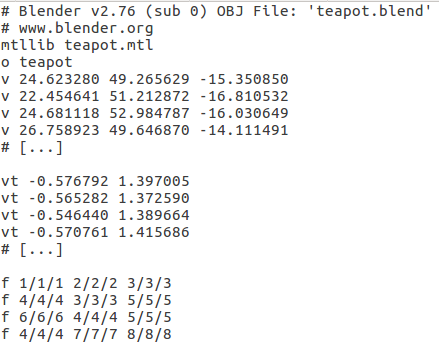
\includegraphics[width=.6\textwidth]{obj_content.png}\\ % PNG-File
  \caption{Notation in .OBJ format}\label{fig:obj_content}
\end{figure}

All these types of information share the following properties which were of relevance for this work. They are contiguous lists of lines, each line representing one instance of the data type indicated in the beginning of the line. Figure \ref{fig:obj_content} depicts an excerpt of an .OBJ file ocntaining vertices (lines starting with v), vertex texture coordinates (lines starting wit vt) and faces (lines starting with f).

These lists are not ordered. Depending on the modelling process, the vertices, faces and all the other attributes can be presented in an completely arbitrary order which hold very little information about the actual, geometric features of the object. The spatial position of any given vertex in relation to the entire object can not be retrieved from this type of notation. This created the demand for spatially indexing of 3D data in the scope this work.

I decided to implement the concept of Octrees \cite{Octree} because of its convenient characteristics as well as prior, personal working experience with \textit{quadtrees}. In an octree, the geometric size of the smallest possible leaf node can be determined in direct relation to the object to be indexed and, at any level, all leafs and nodes will be of the same size. This is highly useful in radius-based proximity-requests for multipl reasons as described in section \ref{sec:addVerticesToSelectionByCoordinates()}.

\begin{figure}[htb]
  \centering
  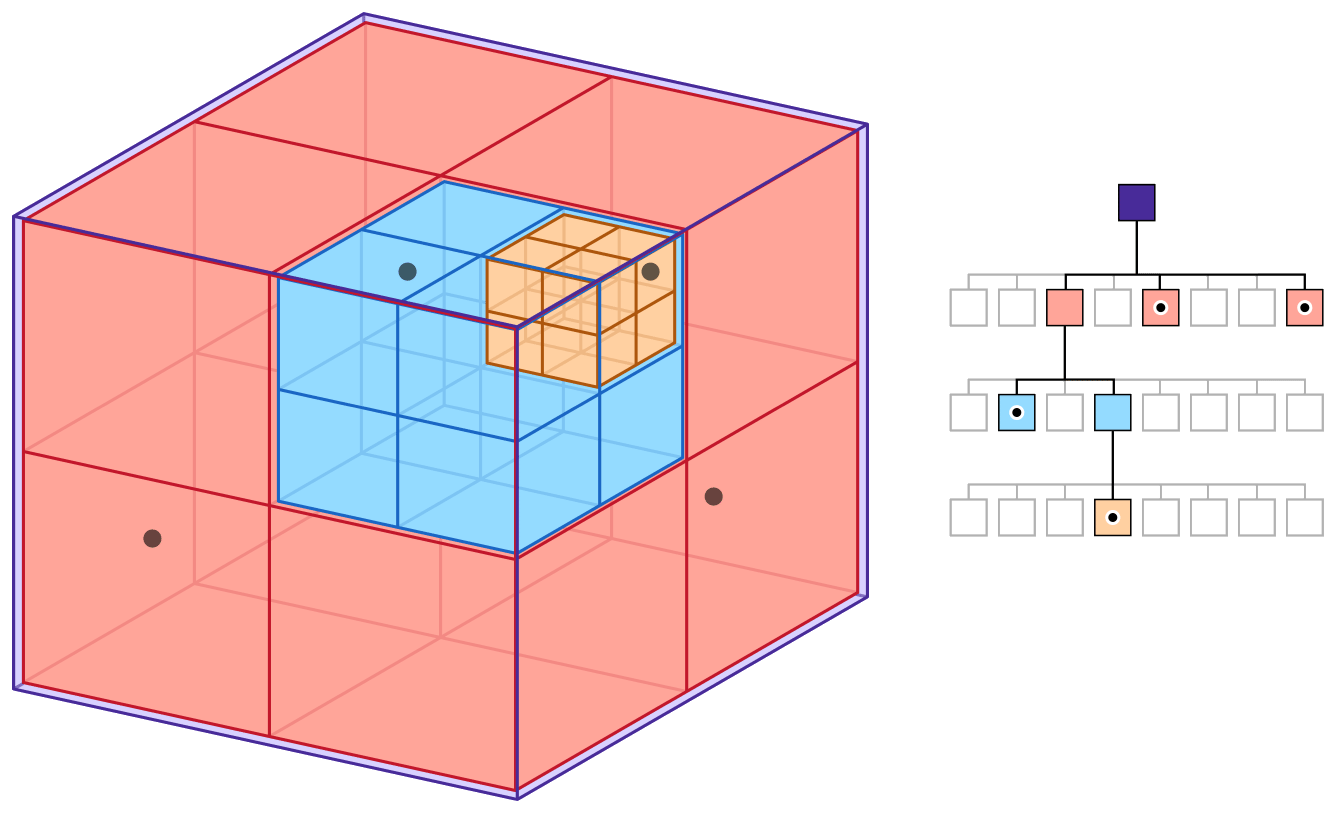
\includegraphics[width=.9\textwidth]{ocTree_apple.png}\\ % PNG-File
  \caption{An octree structure indexing four vertices. Left: 3D view, right: tree structure; 2017, https://developer.apple.com/documentation/}\label{fig:ocTree_apple}
\end{figure}

One of the most common queries performed on 3D data are proximity queries. This means that vertices located within a given radius around an input query-coordinate are to be retrieved. The trivial and obviously highly inefficient solution to such a problem would be to iterate through the entire list of vertices and their coordinates and check for those who fulfill this query condition. This is where spatial indexing structures such ad octree come into play. The concept of octrees is highly recursive and can realize all the most common types of queries (including search queries) in logarithmic time.

An octree is a set of nodes that store references to one another. The highest-level node is called the root node, bottom level nodes are usually referred to as leaf nodes or leafs. Every node that is not a leaf node has eight children-nodes which, in a spatial sense, make up the entire space of their parent node. Such non-leaf nodes can also be described as roots of subtrees.

Figure \ref{fig:ocTree_apple} taken from \cite{octAp} shows a simple octree structure indexing four vertices, both in 3D and tree view. Note how the root node on level 0, shaded purple on the right, is represented as a large purple cube on the left, encompassing the entire set of vertices. The figure clearly visualizes how an non-balanced octree structure that allows one vertex per leaf node at most would look like. On levels 1, 2 and 3, there are eight nodes each. On level 1, there are two leaf nodes that hold one vertex each, on level 2 and 3, there is one leaf holding one vertex each.

The most important parameter for an octree is the maximum allowed number of vertices per leaf node. Once the dimensions in x-,y - and z-direction of the 3D object to be indexed have been determined, the root node of the octree will store every vertex until said maximum allowed number of vertices is reached. Up until that point, the root node was still a leaf. It is now a root no longer and will create eight new nodes (its child nodes) and store references to them. This process is repeated for recursively for every new node until every leaf node holds less than the maximum allowed number of vertices per leaf node. Note that in many implementations of the octree concept, every leaf node needs to be at the same level. For this work, I decided to implement the non-balanced version of an octree where this is not the case.

		\subsection{Selection process}
		\label{sec:selection_process}

To gather data to compare with computer generated mesh saliency maps, tracking user input was needed. In the five-sided projection installation of the \cite{v2c}, 3D objects would be loaded and spatially indexed using octrees as described in the section above. Now, the selection function had to be implemented. Using a handheld input device, a so-called \textit{wand}, as depicted in figure \ref{fig:wand}, users can interact with the scene in two essential ways - navigation and performing arbitrary operations mapped to the device's buttons. Each such operation can, among other information, use the current position and rotation of the wand as parameters.

%  @TODO: Richtiges Foto 1fuegen
\begin{figure}[htb]
  \centering
  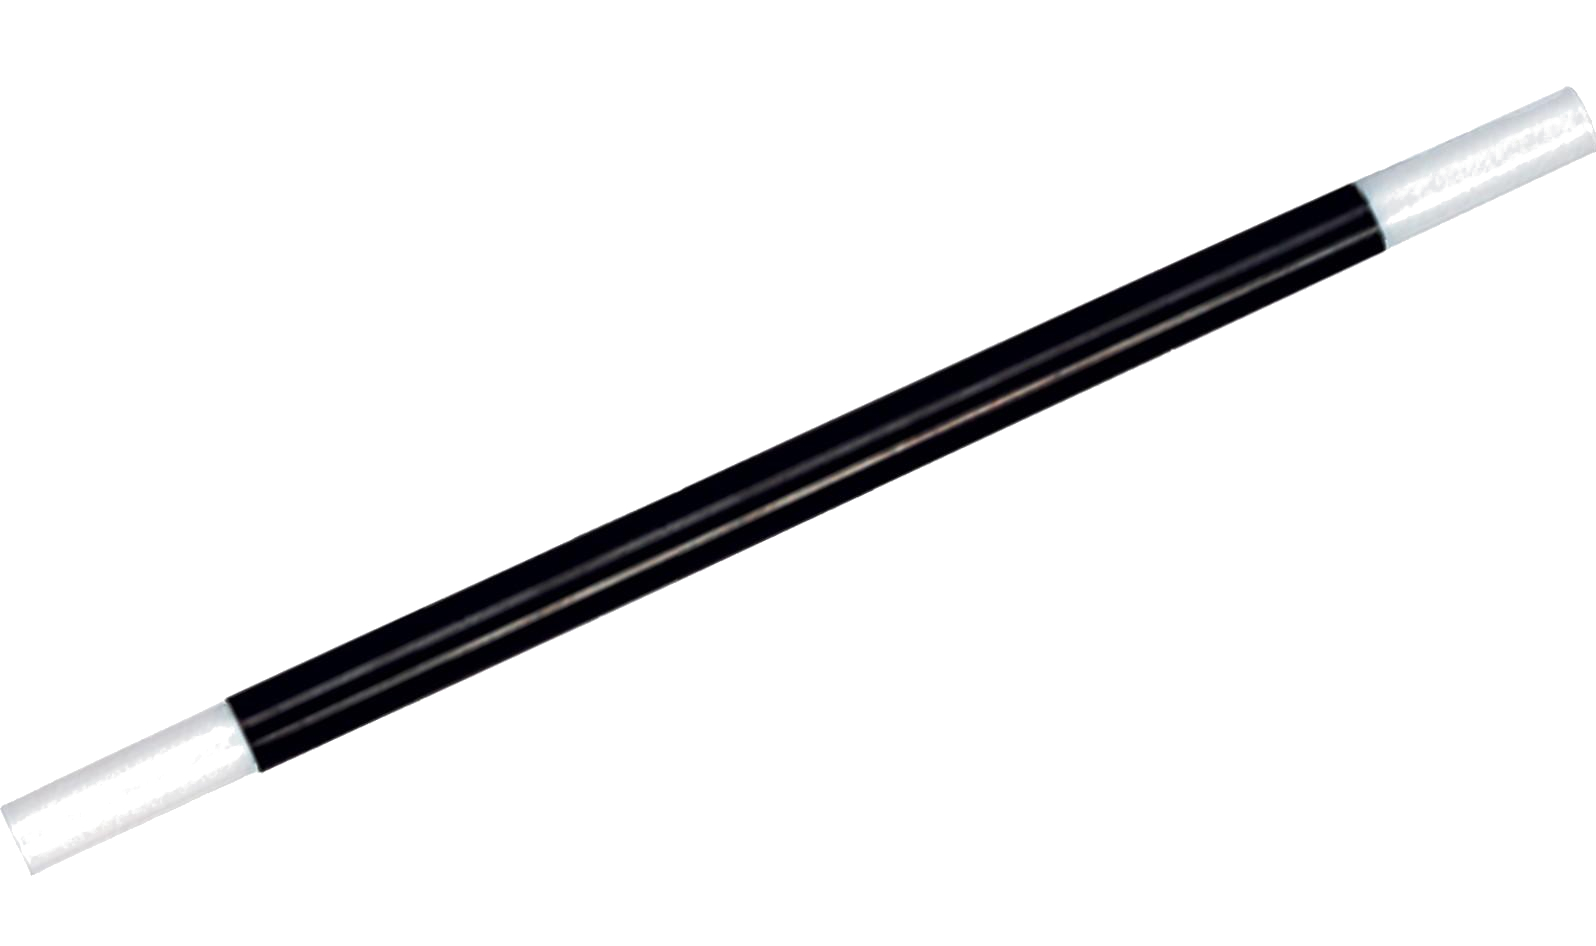
\includegraphics[width=.75\textwidth]{placeholder/wand.jpg}\\ % PNG-File
  \caption{The input device used at the V2C}\label{fig:wand}
\end{figure}

Figure \ref{fig:wand} depicts the \textit{wand} used in the V2C. The little yellow joystick in the middle of its top side, in combination with the current rotation of the device, can be used to navigate the user's view onto the scene. Two of the the three buttons in front of the joystick are mapped to essential functions of the application: The (from the perspective of a user holding the \textit{wand}) left button adds vertices near the current position of the wand to the vertex selection and the righthand button removes such vertices from it. The button in the middle does not have a function in this application, as well as the trigger-like fourth button on the button side of the \textit{wand} (not in view in the figure).
In accordance with the simplistic structure of the user study, the interaction was designed to be as little complex as possible, hence only these two buttons having actual, distinct purposes. 

With this setup in place, everything needed to implement the user selection part of the application is at hand. In order to provide as much visual accuracy as possible, a bright green diamond shaped object at the tracked position of the \textit{wand} is projected into the scene in addition to the loaded model. To additionally provide clear visual feedback, vertices selectes are painted in bright red, clearly seperating them from non-selected parts of the object, displayed in plain grey. For more details on the visual presentation of the application, see 
% @TODO Verweis auf Kapitel User Study bzw. den Teil wo Fotos sind 1bauen

Whenever a user presses the left button of the \textit{wand}, a proximity query is performed on the octree structure indexing the object with its current position as the input. The position is passed as a \texttt{glm::vec3} variable, a basic 3D vector type provided by openGL's mathematics library. For a detailed description of how such a query is handled in this application, see section \ref{sec:addVerticesToSelectionByCoordinates()}.

In addition to these input coordinates, the following two parameters are passed to calls to this function in the context of a user adding or removing vertices to the current selection. The pre-computed selection radius as a \texttt{float} value and a reference to a temporary set of \texttt{size\_t} values called \texttt{intermediateSelection}, holding unique vertex IDs. After a query is terminated, the set of vertices found will be added to this temporary set.
Due to the design of the synchronisation routine between the server and the client threads of this application, this set will be emptied before the result of each such query is returend and written to it. If the \textit{add} button was pressed, the content of \texttt{intermediateSelection} will be added to another set holding the list of currently selected vertices total. If the \textit{remove} button was pressed, each of the temporarily selected vertices will be looked up in this second set and, in case it is found, removed from it. This approach prevents the total set of selected vertices to be sent from the server to all client threads at every frame during runtime. Only newly selected vertices (or those that are to be removed from the current selection) are sent across the application. The time for each action (in seconds since the application was started) is logged as well. 

	\section {Conduct user study with the selection application}
	\label{sec:conduct_user_study_with_the_selection_application}
% generell beschreiben (Aufbau, Ziel, Zusammenhang mit vorigen Sections), Details in eigenem grossen Kapitel
The essential part of this work was conducting a user study where all of the aspects described in this chapter so far would be put to use. The goal was to collect data on what parts of 3D objects users found visually interesting or important. Users put on the stereoscopic, trackable glasses depicted in figure \ref{fig:glasses}, stepped inside the five-sided projection installation of the \cite{v2c} and were asked to mark regions of the object currently displayed that they considered to be intersting or important. The exact wording of the task given to participants in the user study reads as follows.
% @TODO Genau die Fragen / Aufgaben formulieren, textit{please go 14/17 usw}

%  @TODO: Richtiges Foto 1fuegen
\begin{figure}[htb]
  \centering
  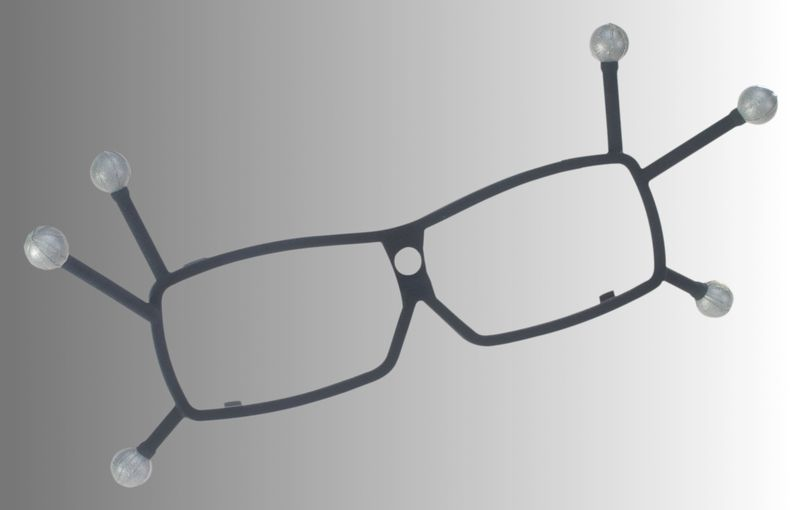
\includegraphics[width=.75\textwidth]{placeholder/glasses_tracked_stereoscopic.jpg}\\ % PNG-File
  \caption{The trackable, stereoscopic glasses used at the V2C}\label{fig:glasses}
\end{figure}

Selections of the users would be gathered to compute user-weighted importance maps for the displayed 3D objects. These would be compared to previously computed mesh saliency maps. For the results and discussion of this comparison, see chapter 
% @TODO ref zu chapter "results usw" 1fügen. Selbiges davor noch anlegen

	\section {Measure of differences}
	\label{sec:measure_of_difference}
% Mit Details, Formelns & Pseudo-Code beschreiben, hierauf dann im "Auswertung sonstwas" chapter verweisen
Since a large portion of the workload of this work was the implementation of the selection application itself, as well as customizing it to the point it is executable in the V2C, the comparison of user generated and pre-computed mesh saliency maps was designed to be quick and easy. In this chapter I will describe how I conceptualised and a basic way to compute a \textit{difference ratio}, normalised to a decimal value between 0 and 1, describing how much user saliency maps differ from mesh saliency maps. It is based on a simple vertex-wise comparison of saliency-values and makes use of the proximity queries provided by the octree structure that is also the basis for the selection application itself as described in section \ref{sec:spatial_indexing_via_octree}.
% @TODO Mail an Markus rauskramen und uebernehmen was ich da geschrieben hab. Vielleicht lustige Bilders machen

In chapter % @TODO ref zu chapter "results usw" 1fügen. Selbiges davor noch anlegen
I consider both \textit{raw} and \textit{weighted difference} values.

